
%\ed{> Part IV describes in great detail Multipath TCP and TCP Minion,
%two recent significant evolutions of TCP that were built with
%deployability in mind. \textbf{Multipath TCP - Costin (10 pages)}}

Today's networks are multipath: mobile devices have multiple wireless
interfaces, datacenters have many redundant paths between servers and
multi-homing has become the norm for big server farms. Meanwhile, TCP
is essentially a single path protocol: when a TCP connection is
established, it is bound to the IP addresses of the two communicating
hosts. If one of these addresses changes, for whatever reason, the
connection fails. In fact a TCP connection cannot even be
load-balanced across more than one path within the network, because
this results in packet reordering and TCP misinterprets this
reordering as congestion and slows down.

This mismatch between today's multipath networks and TCP's single-path
design creates tangible problems. For instance, if a smartphone's WiFi interface
loses signal, the TCP connections associated with it stall - there is
no way to migrate them to other working interfaces, such as 3G. This
makes mobility a frustrating experience for users.  Modern datacenters
are another example: many paths are available between two endpoints,
and equal cost multipath routing randomly picks one for a particular TCP
connection.  This can cause collisions where multiple flows get placed
on the same link, hurting throughput - to such an extent that average 
throughput is halved in some scenarios.

Multipath TCP (MPTCP) \cite{rfc6284} is a major modification to TCP that allows multiple
paths to be used simultaneously by a single 
connection. Multipath TCP circumvents the issues above and several
others that affect TCP.  Changing TCP to use multiple paths is not a
new idea: it was originally proposed more than fifteen years ago by
Christian Huitema in the Internet Engineering Task Force (IETF) \cite{Huitema_Multi-homed:1995}, and
there have been a half-dozen more proposals since then to similar
effect. Multipath TCP draws on the experience gathered in previous
work, and goes further to solve issues of fairness when competing with
regular TCP and deployment issues due to middleboxes in today's
Internet. 

\subsection{Overview of Multipath TCP}

The design of Multipath TCP has been influenced by many requirements,
but there are two that stand out: application compatibility and
network compatibility. Application compatibility implies that 
applications that today run over TCP should work without any change 
over Multipath TCP. Next, Multipath TCP must
operate over any Internet path where the TCP protocol operates.

As explained earlier, many paths on today's Internet include middleboxes that, unlike routers,
 know about the TCP connections they forward, and affect them in special ways. 
Designing TCP extensions that can safely traverse all these middleboxes has
proven to be challenging.

Multipath TCP allows multiple "subflows" to be combined to form a single MPTCP
session.  An MPTCP session starts with an initial subflow which is
very similar to a regular TCP connection, with a three way handshake.  After
the first MPTCP subflow is set up, additional subflows can be
established.  Each subflow also looks very similar to a
regular TCP connection, complete with three-way handshake and graceful tear-down,
but rather than being a separate connection it is bound into an
existing MPTCP session.  Data for the connection can
then be sent over any of the active subflows that has the capacity to
take it.

To examine Multipath TCP in more detail, let us consider a very simple
scenario with a smartphone client and a single-homed server. The
smartphone has two network interfaces: a WiFi interface and a 3G
interface; each has its own IP address.  The server, being
single-homed, has a single IP address. In this environment, Multipath
TCP would allow an application on the mobile device to use a single MPTCP
session that can use both the WiFi and the 3G interfaces to
communicate with the server.  The application opens a regular TCP socket, and
the kernel enables MPTCP by default if the remote end supports it, using both paths. 
The application does not need to concern itself with which radio interface is working best at any instant;
MPTCP handles that for it. In fact, Multipath TCP can work when
both endpoints are multihomed (in this case subflows are opened between
all pairs of "compatible" IP addresses), or even in the case when 
both endpoints are single homed (in this case different subflows will use
 different port numbers, and can be routed differently by multipath routing 
in the network). 

\paragraph{Connection Setup.} Let us walk through the establishment of an MPTCP connection. 
Assume that the mobile device chooses its 3G interface to open the
connection. It first sends a \texttt{SYN} segment to the server. This segment
contains the \texttt{MP\_CAPABLE} TCP option indicating that the mobile device
supports Multipath TCP. This option also contains a key which is
chosen by the mobile device. The server replies with a \texttt{SYN+ACK} segment
containing the \texttt{MP\_CAPABLE} option and the key chosen by the server. The
mobile device completes the handshake by sending an \texttt{ACK} segment.

The initial MPTCP connection setup is shown graphically in the top part of Figure \ref{fig:mptcp_handshake},
where the segments are regular TCP segments carrying new multipath TCP-related options (shown in green).

\begin{figure}[t]
\centering
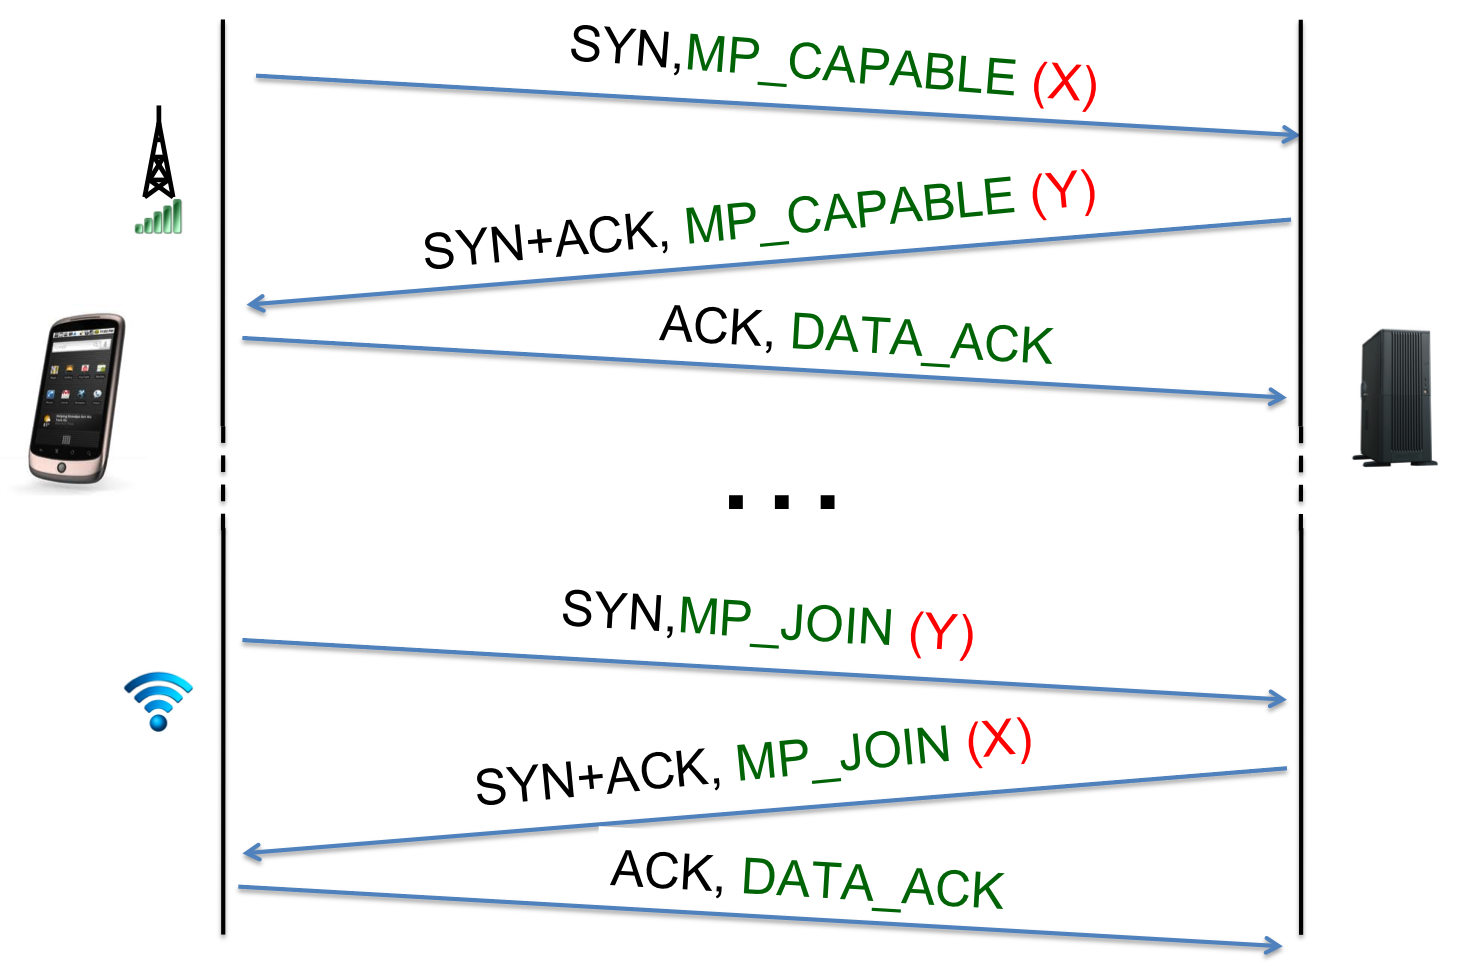
\includegraphics[width=0.9\textwidth]{figures/mptcp_handshake.png}
\caption{Multipath TCP handshake: multiple subflows can be added and removed after the initial
connection is setup and connection identifiers are exchanged.}
\label{fig:mptcp_handshake}
\end{figure}

At this point the Multipath TCP connection is established and the
client and server can exchange TCP segments via the 3G path. How
could the mobile device also send data through this Multipath TCP
session over its WiFi interface?

Naively, it could simply send some of the segments over the WiFi
interface.  However most ISPs will drop these packets, as they would
have the source address of the 3G interface.  Perhaps the client could
tell the server the IP address of the WiFi interface, and use that
when it sends over WiFi?  Unfortunately this will rarely work:
firewalls and similar stateful middleboxes on the WiFi path expect to
see a \texttt{SYN} segment before they see data segment.  The only solution that
will work reliably is to perform a regular three-way handshake on the WiFi path
before sending any packets that way, so this is what Multipath TCP
does.  This handshake carries the \texttt{MP\_JOIN} TCP option, providing
information to the server that can securely identify the
correct connection to associate this additional subflow with.  The
server replies with \texttt{MP\_JOIN} in the \texttt{SYN+ACK}, and the new subflow is
established (this is shown in the bottom part of Figure \ref{fig:mptcp_handshake}). 

An important point about Multipath TCP, especially in the context of 
mobile devices, is that the set of subflows that are associated to a Multipath TCP 
connection is not fixed. Subflows can be dynamically added and removed from a 
Multipath TCP connection throughout its lifetime, without affecting the 
bytestream transported on behalf of the application. 
If the mobile device moves to another WiFi network, it will receive a new IP 
address. At that time, it will open a new subflow using its newly allocated address 
and tell the server that its old address is not usable anymore. The server will now 
send data towards the new address. These options allow mobile devices to easily move
through different wireless connections without breaking their
Multipath TCP connections \cite{Paasch_Mobile:2012}.

Multipath TCP also implements mechanisms that allows to inform the
remote host of the addition/removal of addresses even when an endpoint operates behind a NAT, or when a subflow using a
different address family is needed (e.g. IPv6). Endpoints can send
an \texttt{ADD\_ADDR} option that contains an address identifier together with an address.
The address identifier is unique at the sender, and allows it to identify its addresses
even when it is behind a NAT. Upon receiving an advertisement, the endpoint may initiate a new subflow to
the new address. An address withdrawal mechanism is also provided via the \texttt{REMOVE\_ADDR}
option that also carries an address identifier. 

\paragraph{Data Transfer.} Assume now that two subflows have been established over WiFi and 3G:
the mobile device can send and receive data segments over both. Just like TCP, Multipath
TCP provides a bytestream service to the application.  In
fact, standard applications can function over MPTCP without being
aware of it - MPTCP provides the same socket interface as TCP.

Since the two paths will often have different delay characteristics,
the data segments sent over the two subflows will not be received in
order. Regular TCP uses the sequence number in the TCP header
to put data back into the original order. A simple solution for
Multipath TCP would be to just reuse this sequence number as
is. 

Unfortunately, this simple solution would create problems with
some existing middleboxes such as firewalls. On each path, a middlebox
would only see half of the packets, so it would observe many gaps in
the TCP sequence space. Measurements indicate that some middleboxes
react in strange ways when faced with gaps in TCP sequence
numbers \cite{honda2011still}. Some discard the out-of-sequence segments while others try to
update the TCP acknowledgments in order to "recover" some of these
gaps. With such middleboxes on a path, Multipath TCP cannot safely
send TCP segments with gaps in the TCP sequence number space. On the
other hand, Multipath TCP also cannot send every data segment over all
subflows: that would be a waste of resources.

To deal with this problem, Multipath TCP uses its own sequence
numbering space.  Each segment sent by Multipath TCP contains two
sequence numbers: the subflow sequence number inside the regular TCP
header and an additional Data Sequence Number (DSN). 


This solution ensures that the segments sent on any given
subflow have consecutive sequence numbers and do not upset
middleboxes.  Multipath TCP can then send some data sequence numbers
on one path and the remainder on the other path; the DSN will be used by the Multipath TCP
receiver to reorder the bytestream before it is given to the receiving
application.

Before we explain the way the Data Sequence Number is encoded, we first need to discuss two other
key parts of Multipath TCP  that are affected by the additional sequence number
space---flow control and acknowledgements.

\paragraph{Flow Control.}
TCP's receive window indicates the number of bytes beyond the sequence number from the acknowledgment field that the receiver 
can buffer. The sender is not permitted to send more than this amount of additional data.
Multipath TCP also needs to implement flow control, although segments
can arrive over multiple subflows. If we 
inherit TCP's interpretation of receive window, this would imply an MPTCP receiver maintains a pool of buffering 
per subflow, with receive window indicating per-subflow buffer occupancy. Unfortunately such an interpretation 
can lead to deadlocks:
\begin{enumerate}
\item The next segment that needs to be passed to the application was
  sent on subflow 1, but was lost.
\item In the meantime subflow 2 continues delivering data, and fills
  its receive window.
\item Subflow 1 fails silently.
\item The missing data needs to be re-sent on subflow 2, but there is
  no space left in the receive window, resulting in a deadlock.
\end{enumerate}

The correct solution is to generalize TCP's receive window semantics to MPTCP. For each connection \emph{a 
single receive buffer pool should be shared between all subflows}. The receive window then indicates 
the maximum data sequence number that can be sent rather than the maximum subflow sequence number. As 
a segment resent on a different subflow always occupies the same data sequence space, deadlocks cannot occur.

The problem for an MPTCP sender is that to calculate the highest data sequence number that can be sent, 
the receive window needs to be added to the highest data sequence number acknowledged. However the ACK 
field in the TCP header of an MPTCP subflow must, by necessity,
indicate only subflow sequence numbers to cope with middleboxes. 
Does MPTCP need to add an extra data acknowledgment field for the receive window to be interpreted correctly?

\paragraph{Acknowledgments.} 
The answer is positive: MPTCP needs and uses \emph{explicit
connection-level acknowledgments} or \emph{DATA\_ACKs}. The alternative is to infer connection-level
acknowledgments from subflow acknowledgments, by using a scoreboard maintained by the sender that maps
subflow sequence numbers to data sequence numbers. Unfortunately, MPTCP segments and their associated ACKs
will be reordered as they travel on different paths, making it impossible to correctly infer the connection-level
acknowledgments from subflow-level ones \cite{raiciu2012hard}.

\paragraph{Encoding.}
We have seen that in the forward path we need to encode a mapping of
subflow bytes into the data sequence space, and in the reverse path we
need to encode cumulative data acknowledgments.  There are two viable
choices for encoding this additional data:
\begin{itemize}
\item Send the additional data in TCP options.
\item Carry the additional data within the TCP payload, using a
  chunked or escaped encoding to separate control data from payload
  data.
\end{itemize}

For the forward path there aren't compelling arguments either
way, but the reverse path is a different matter.
Consider a hypothetical encoding that divides the payload into chunks
where each chunk has a TLV (type-length-value) header.  A data acknowledgment can then be
embedded into the payload using its own chunk type.  Under most
circumstances this works fine.  However, unlike TCP's pure ACK, anything
embedded in the payload must be treated as data.  In particular:
\begin{itemize}
\item It must be subject to flow control because the receiver must
  buffer data to decode the TLV encoding.

\item If lost, it must be retransmitted consistently, so that
  middleboxes can track sequence state correctly\footnote{TCP proxies re-send the original
    content they see a ``retransmission'' with different data. }
\item If packets before it are lost, it might be necessary to wait for retransmissions
  before the data can be parsed - causing head-of-line blocking. 
%\item The packet it is contained in may be split into two packets or
%  merged with other packets by middleboxes or TCP segmentation offload hardware.
\end{itemize}

%This last issue does not greatly affect MPTCP at present.  We observed
%3\% of paths coalesced segments (7\% on port 80) and 3\% of paths also
%split segments (7\% on port 80).  However almost all of these removed {\sc
%  Mp\_Capable} from the \SYNs, so MPTCP would not be enabled.  We did
%however observe one middlebox that passed {\sc Mp\_Capable} and
%resegmented data, but only when no new options were present in data
%packets - this might affect MPTCP if chunked payload encoding were used.

\begin{figure}[t]
\centering
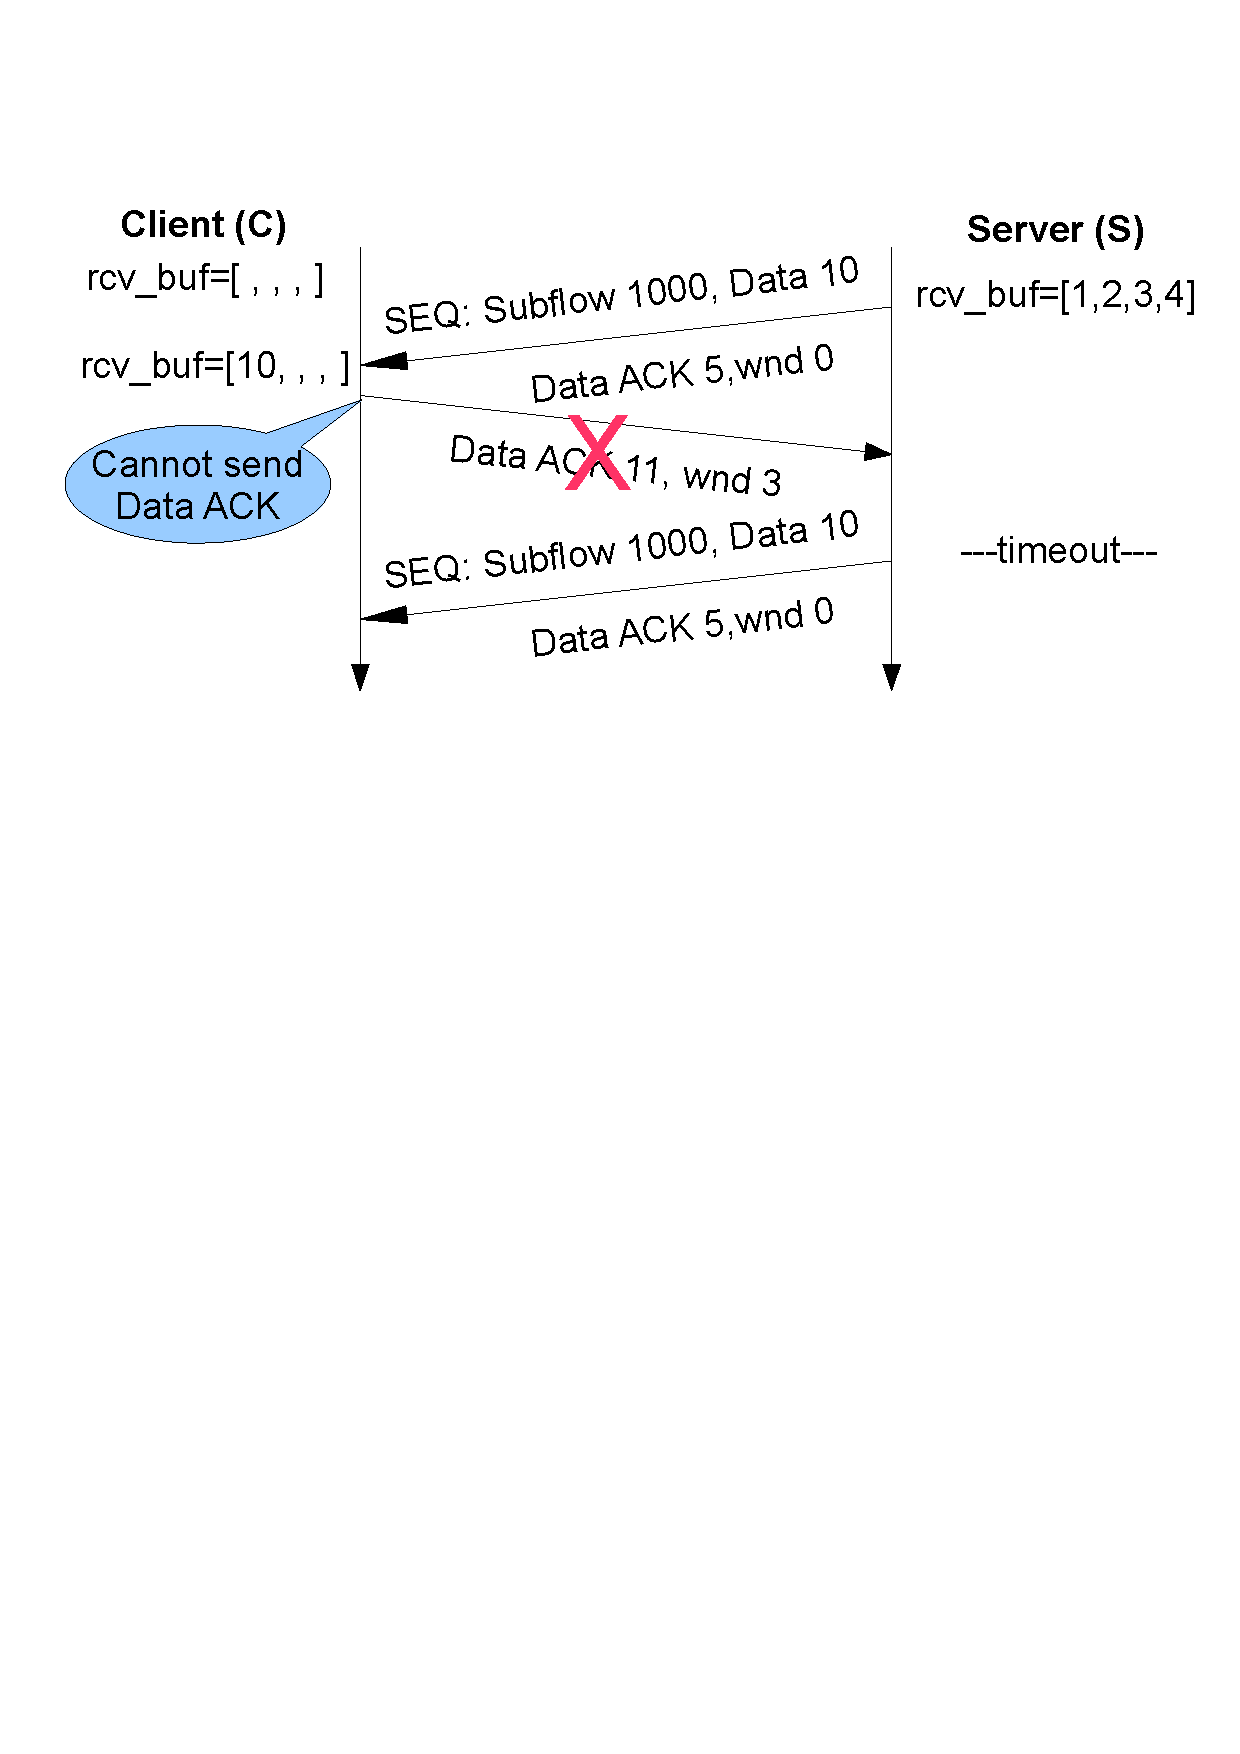
\includegraphics[trim=1cm 17cm 1cm 1cm,clip=true,height=6cm]{figures/dataack_deadlock}
\caption{Flow Control on the path from C to S inadvertently stops the data flow from S to C}
\label{fig:dack_deadlock}
\end{figure}

Flow control presents the most obvious problem for the
chunked payload encoding.  Figure \ref{fig:dack_deadlock} provides an
example. Client C is pipelining requests to server S; meanwhile S's
application is busy sending the large response to the first request so
it isn't yet ready to read the subsequent requests.  At this point,
S's receive buffer fills up.

S sends segment 10, C receives it and wants to send the \texttt{DATA\_ACK}, but
cannot: flow control imposed by S's receive window stops him.
Because no \texttt{DATA\_ACK}s are received from C, S cannot free his send
buffer, so this fills up and blocks the sending application on S.  S's
application will only read when it has finished sending data to C, but
it cannot do so because its send buffer is full.  The send buffer can
only empty when S receives the \texttt{DATA\_ACK} from C, but C cannot send this 
until S's application reads.  This is a classic deadlock cycle.
As no \texttt{DATA\_ACK} is received, S will eventually time out the data it
sent to C and will retransmit it;  after many retransmits the whole connection will time out.

The conclusion is that \texttt{DATA\_ACK}s cannot be safely encoded in the
payload.  The only real alternative is to encode them in TCP options
which (on a pure ACK packet) are not subject to flow control.  

\paragraph{The Data Sequence Mapping.} 
If MPTCP must use options to encode \texttt{DATA\_ACK}s, it is simplest to also
encode the mapping from subflow sequence numbers to data sequence
numbers in a TCP option.  This is the {\em data sequence
mapping} or DSM.

At first glance it seems the {\sc DSM} option simply needs to carry the data
sequence number corresponding to the start of the MPTCP segment.
Unfortunately middleboxes and interfaces that implement TSO or LRO make this far from
simple.  

Middleboxes that re-segment data would cause a problem.
TCP Segmentation Offload (TSO) hardware in the
network interface card (NIC) also re-segments data and is commonly used to improve performance.
The basic idea is that the OS sends large segments and the NIC 
re-segments them to match the receiver's MSS.  What does TSO do 
with TCP options?  A test of 12 NICs supporting
TSO from four different vendors showed that all of them copy a TCP option sent
by the OS on a large segment into all the split segments \cite{raiciu2012hard}.

If MPTCP's DSM option only listed the data sequence number, TSO would
copy the same DSM to more than one segment, breaking the mapping.
Instead the DSM option must say precisely which subflow bytes map to
which data sequence numbers.  But this is further complicated by
middleboxes that modify the initial sequence number of TCP connections
and consequently rewrite all sequence numbers (many firewalls behave like this).
Instead, the {\sc DSM} option must map the offset from the
subflow's initial sequence number to the data sequence number, as the
offset is unaffected by sequence number rewriting.  The option must
also contain the length of the mapping.  This is robust - as long as
the option is received, it does not greatly matter which packet
carries it, so duplicate mappings caused by TSO are not a
problem.

\paragraph{Dealing with Content-Modifying Middleboxes.}
Multipath TCP and content-modifying middleboxes (such as application-level NATs, e.g. for FTP)
have the potential to interact badly.  In particular, due to FTP's ASCII
encoding, re-writing an IP address in the payload can necessitate
changing the length of the payload.  Subsequent sequence and ACK
numbers are then fixed up by the middlebox so they are consistent from
the point of view of the end systems.

Such length changes break the DSM option mapping - subflow bytes can
be mapped to the wrong place in the data stream.  They also
break every other possible mapping mechanism, including chunked
payloads.  There is no easy way to handle such middleboxes.

That is why MPTCP includes an optional checksum in
the DSM mapping to detect such content changes. If an MPTCP host
receives a segment with an invalid DSM checksum, it
rejects the segment and triggers a fallback process:  if any
other subflows exists, MPTCP terminates the subflow on which the
modification occurred;  if no other subflow exists, MPTCP drops back to
regular TCP behavior for the remainder of the connection, allowing the
middlebox to perform rewriting as it wishes. This fallback mechanism
preserves connectivity in the presence of middleboxes.

For efficiency reasons, MPTCP uses the same 16-bit ones complement checksum
used in the TCP header.  This allows the checksum over the payload to
be calculated only once.  The payload checksum is added to a checksum
of an MPTCP pseudo header covering the DSM mapping values and then
inserted into the DSM option.   The same payload checksum is added to the
checksum of the TCP pseudo-header and then used in the TCP checksum field.
MPTCP allows checksums to be disabled for high performance environments such as data-centers where
there is no chance of encountering such an application-level gateway.

The fall-back-to-TCP process, triggered by a checksum failure, can also
be triggered in other circumstances.  For example, if a routing
change moves an MPTCP subflow to a path where a middlebox
removes DSM options, this also triggers the fall-back procedure.


\begin{figure}[t]
\centering
\begin{verbatim}
                      1                   2                   3
  0 1 2 3 4 5 6 7 8 9 0 1 2 3 4 5 6 7 8 9 0 1 2 3 4 5 6 7 8 9 0 1
 +---------------+---------------+-------+----------------------+
 |     Kind      |    Length     |Subtype| (reserved) |F|m|M|a|A|
 +---------------+---------------+-------+----------------------+
 |           Data ACK (4 or 8 octets, depending on flags)       |
 +--------------------------------------------------------------+
 |   Data Sequence Number (4 or 8 octets, depending on flags)   |
 +--------------------------------------------------------------+
 |              Subflow Sequence Number (4 octets)              |
 +-------------------------------+------------------------------+
 |  Data-level Length (2 octets) |      Checksum (2 octets)     |
 +-------------------------------+------------------------------+
\end{verbatim}
\caption{The Data Sequence Signal option in MPTCP that carries the Data Sequence Mapping information,
the Data ACK, the Data FIN and connection-fall-back options. }
\label{fig:mptcp_dss}
\end{figure}

\paragraph{Connection Release.} Multipath TCP must allow a connection to survive
even though its subflows are coming and going. Subflows in MPTCP can be torn down
by means of a four-way handshake as regular TCP flows---this ensures MPTCP
allows middleboxes to clear their state when a subflow is not used anymore.

MPTCP uses an explicit four-way handshake for connection tear-down indicated by a \texttt{DATA\_FIN} option.
The \texttt{DATA\_FIN} is MPTCP's equivalent to TCP's \texttt{FIN}, and it occupies one byte in the data-sequence 
space. A \texttt{DATA\_ACK} will be used to acknowledge the receipt of the \texttt{DATA\_FIN}. MPTCP requires
that the segment(s) carrying a \texttt{DATA\_FIN} must also have the \texttt{FIN} flag set - this ensures
all subflows are also closed when the MPTCP connection is being closed.

For reference, we show the wire format of the option used by MPTCP for data exchange in Figure 
\ref{fig:mptcp_dss}. This option encodes the Data Sequence Mapping, Data ACK, Data FIN and 
the fall-back options. The flags specify which parts of the option are valid, and help reduce option
space usage. 

\subsection{Congestion Control}

One of the most important components in TCP is its congestion controller which 
enables it to adapt its throughput dynamically in response to changing network 
conditions. To perform this functionality, each TCP sender maintains a congestion 
window $w$ which governs the amount of packets that the sender can send without 
waiting for an acknowledgment. The congestion window is updated dynamically 
according to the following rules:

\begin{itemize}
\item On each ACK, increase the window $w$ by $1/w$.
\item Each loss decrease the window $w$ by $w/2$.
\end{itemize}

TCP congestion control ensures fairness:  when multiple connections 
utilize the same congested link each of them will independently converge to the 
same average value of the congestion window.  

What is the equivalent of TCP congestion control for multipath
transport? The obvious question to ask is why not just run regular TCP congestion
control on each subflow?
Consider the scenario in Fig. \ref{fig:1bottleneck}. If multipath
TCP ran regular TCP congestion control on both paths, then the
multipath flow would obtain twice as much throughput as the single
path flow (assuming all RTTs are equal). This is unfair. To solve
this problem, one solution is to try and detect shared bottlenecks
but that is unreliable; a better solution is be less aggressive on
each subflow (i.e. increase window slower) such that in aggregate the MPTCP connection 
is no more aggressive than a single regular TCP connection. 


Before we describe solutions to MPTCP congestion control, let's discuss the three goals that
multipath congestion control must obey \cite{mptcp-cc}:
\begin{enumerate}
\item[\textbf{Fairness}] If several subflows of the same MPTCP connection
share a bottleneck link with other TCP connections, MPTCP should not
get more throughput than TCP. 
\item[\textbf{Deployability}] The performance of all the
Multipath TCP subflows together should be at least that of regular TCP
on any of the paths used by a Multipath TCP connection.  This ensures
that there is an incentive to deploy Multipath TCP. 
\item[\textbf{Efficiency}] A final, most important goal is that Multipath TCP should prefer efficient paths,
which means it should send more of its traffic on paths experiencing
less congestion.
\end{enumerate}

\begin{figure}[t]
\centering
\includegraphics*[width=0.45\columnwidth,bb=167 245 509 380]{figures/1bottleneck}
\caption{A scenario which shows the importance of weighting the
  aggressiveness of subflows (Reprinted from \cite{mptcp-cc}. Included
  here by permission).}
\label{fig:1bottleneck}
\end{figure}

\begin{figure}[t]
\centering
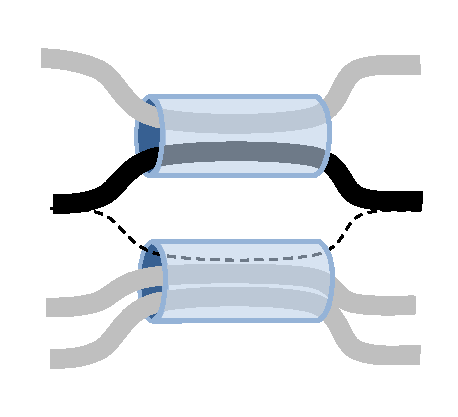
\includegraphics[width=0.5\textwidth]{figures/figure1}
\caption{Two links each with capacity 20~pkts/s. The top link is used by a single TCP connection,
and the bottom link is used by two TCP connections. A Multipath TCP connection uses
both links. Multipath TCP pushes most of its traffic onto less congested top link,
making the two links behave like a resource pool of capacity 40~pkts/s. Capacity is divided equally,
with each flow having throughput 10~pkts/s. (Reprinted from
\cite{mptcp-cc}. Included here by permission)}
\label{fig:mptcp1}
\end{figure}

Intuitively, this last goal ensures wide-area load balancing of traffic: 
when a multipath connection is using two paths loaded unevenly (such as 
Figure \ref{fig:mptcp1}), the multipath transport will prefer the unloaded path
and push most of its traffic there; this will decrease the load on the 
congested link and increase it on the less congested one. 

If a large enough fraction of flows are multipath, congestion will spread 
out evenly across collections of links, creating "resource pools": links 
that act together as if they are a single, larger capacity link shared by 
all flows. This effect is called resource pooling \cite{pooling}.
Resource pooling brings two major benefits, discussed in the paragraphs below.

\paragraph{Increased Fairness.} 
Consider the example shown in Figure \ref{fig:mptcp1}: congestion
balancing ensures that all flows have \textbf{the same throughput}, making
the two links of 20~pkt/s act like a single pooled link with capacity 40~pkt/s 
shared fairly by the four flows. If more MPTCP flows would be added, the two links would still behave as a pool,
sharing capacity fairly among all flows. 
Conversely, if we remove the Multipath TCP flow, the links no longer form a pool, and the throughput allocation
is unfair as the TCP connection using the top path gets twice as much throughput as the TCP connections using the bottom path.


\paragraph{Increased Throughput.}
Consider the somewhat contrived scenario in Fig.\ref{fig:klingon},
and suppose that the three links each have capacity 12Mb/s.
If each flow split its traffic evenly
across its two paths subflow would get 4Mb/s 
hence each flow would get 8Mb/s. But if each flow used only 
the one-hop shortest path, it could get 12Mb/s: this is because
two-hop paths consume double the resources of one-hop paths,
and in a congested network it makes sense to only use the one-hop paths.

\begin{figure}[tb]
\centering
\includegraphics*[width=0.8\columnwidth]{figures/3pipes}
\caption{A scenario to illustrate the importance of choosing the
  less-congested path. (Reprinted from \cite{mptcp-cc}. Included here
  by permission.)}
\label{fig:klingon}
\end{figure}

In an idle network, however, using all available paths is much better: 
consider the case when only the blue connection is using the links. In this
case this connection would get 24Mb/s throughput; using the one hop path
alone would only provide 12Mb/s.

In summary, the endpoints need to be able to dynamically decide 
which paths to use based on conditions in the network. 
A solution has been devised in the theoretical literature on
congestion control, independently by Kelly and Voice \cite{kelly-voice} and
Han et al. \cite{towsley-cc}.  The core idea is that a multipath flow should
shift all its traffic onto the least-congested path.
In a situation like Fig. \ref{fig:klingon} the
two-hop paths will have higher drop probability than the one-hop
paths, so applying the core idea will yield the efficient
allocation.
Surprisingly it turns out that this can be achieved by doing independent
congestion control at endpoints.

\paragraph{Multipath TCP Congestion Control.}
The theoretical work on multipath congestion control \cite{kelly-voice,towsley-cc} assumes a rate-based
protocol, with exponential increases of the rate. TCP, in contrast, is a packet-based
protocol, sending $w$ packets every round-trip time (i.e. the rate is $w/RTT$); 
a new packet is sent only when an acknowledgment is received, confirming that an existing 
packet has left the network. This property is called ACK-clocking 
and is nice because it has good stability properties:
when congestion occurs round-trip times increase (due to buffering), which
\emph{automatically reduces the effective rate} \cite{Jacobson_congestion:88}.


Converting a theoretical rate-based exponential protocol to a practical 
packet-based protocol fair to TCP turned out to be more difficult than expected. 
There are two problems that appear \cite{mptcp-cc}: 
\begin{itemize}
\item When loss rates are equal on all paths, the theoretical algorithm will
place all of the window on one path or the other, not on both---this effect was termed 
``flappiness'' and it appears because of the discrete (stochastic) nature of packet losses which
are not captured by the differential equations used in theory.
\item The ideal algorithm always prefers paths with lower loss rate, but in practice these may have poor
performance. Consider a mobile phone with WiFi and 3G links: 3G links have very low loss rates and huge round-trip
times, resulting in poor throughput. WiFi is lossy, has shorter round-trip times and typically offers much better throughput.
In this common case, a ``perfect'' controller would place all traffic on the 3G path, violating the second goal (deployability).
\end{itemize}

The pragmatic choice is to sacrifice some load-balancing ability to ensure greater stability and
to offer incentives for deployment. This is what Multipath TCP congestion control does.

Multipath TCP congestion control is a series of simple changes to the standard TCP congestion control mechanism. Each subflow 
has its own congestion window, that is halved when packets are lost, as in standard TCP \cite{mptcp-cc}.

Congestion balancing is implemented in the increase phase of 
congestion control: here Multipath TCP will allow less congested subflows 
to increase proportionally more than congested ones. Finally, the total 
increase of Multipath TCP across all of its subflows is dynamically chosen 
in such a way that it achieves the first and second goals above. 

The exact algorithm is described below and it satisfies the goals we've discussed:
\begin{itemize}
\item Upon ACK on subflow $r$, increase the window $w_r$ by
$\min(a/w_{total}),1/w_r)$.
\item Upon loss on subflow $r$, decrease the window $w_r$ by $w_r/2$.
\end{itemize}
Here
\begin{equation}
\label{eq:a}
a = w_{total} \frac{\max_r w_r/RTT_r^2}{(\sum_r
  w_r/RTT_r)^2},
\end{equation}
$w_r$ is the current window size on subflow $r$ and $w_{total}$ is the
sum of windows across all subflows. 

The algorithm biases the increase towards uncongested paths: these will receive
more ACKs and will increase accordingly. However, MPTCP does keep some traffic
even on the highly congested paths; this ensures stability and allows it
to quickly detect when path conditions improve.

$a$ is a term that is computed dynamically upon each packet drop. Its purpose 
is to make sure that MPTCP gets at least as much throughput as TCP on the best path.
To achieve this goal, $a$ is computed by estimating how much TCP would get on each MPTCP path
(this is easy, as round-trip time and loss-rates estimates are known) and ensuring that MPTCP
in stable state gets at least that much. A detailed discussion on the design of the MPTCP congestion
control algorithm is provided in \cite{mptcp-cc}.

For example, in the three-path example above, the flow will put
45\% of its weight on each of the less congested path and 10\% on the
more congested path. This is intermediate between regular TCP
(33\% on each path) and a perfect load balancing algorithm (0\% on the more congested path)
that is impossible to implement in practice.

The window increase is capped at $1/w_r$, which ensures that
the multipath flow can take no more capacity on either path than a
single-path TCP flow would.

In setting the $a$ parameter, Multipath TCP congestion control uses subflow delays to compute the target rate.
Using delay for congestion control is not a novel idea: TCP Vegas \cite{vegas}, for instance, performs
congestion control only by tracking RTT values. Vegas treats increasing RTTs as a sign of congestion, instead
of relying on packet losses as regular TCP does. That is why Vegas loses out to regular TCP at shared bottlenecks,
and is probably the reason for its lack of adoption. MPTCP does not treat delay as congestion: it just uses it
to figure out the effective rate of a TCP connection on a given path. This allows MPTCP to compete fairly with TCP.

\paragraph{Alternative Congestion Controllers for Multipath TCP.} The standardized Multipath
TCP congestion control algorithm chooses a trade-off between load balancing, stability and
the ability to quickly detect available capacity. The biggest contribution of this
work is the clearly defined goals for what multipath congestion control should do,
and an instantiation that achieves (most of) the stated goals in practice.

This research area is relatively new, and it is likely that more work will lead to better 
algorithms---if not generally applicable, then at least tailored to some practical use-cases.
A new and interesting congestion controller called Opportunistic Linked Increases Algorithm (OLIA) 
has already been proposed \cite{olia} that offers better load balancing with seemingly few drawbacks.

We expect this area to be very active in the near future; of particular interest are designing multipath
versions of high-speed congestion control variants deployed in practice, such as Cubic or Compound TCP. 



\subsection{Implementation and performance}

We now briefly cover two of the most compelling use cases for
Multipath TCP by showing a few evaluation results. We focus on mobile
devices and datacenters but note that Multipath TCP can also help in
other scenarios.  For example, multi-homed web-servers can perform
fine-grained load-balancing across their uplinks, while dual-stack
hosts can use both IPv4 and IPv6 within a single Multipath TCP
connection.

The full Multipath TCP protocol has been implemented in the Linux
kernel; its congestion controller has also been implemented in the ns2
and htsim network simulators. The results presented in here are from
the Linux kernel implementation \cite{raiciu2012hard}. 

\begin{figure}[t]
\centering
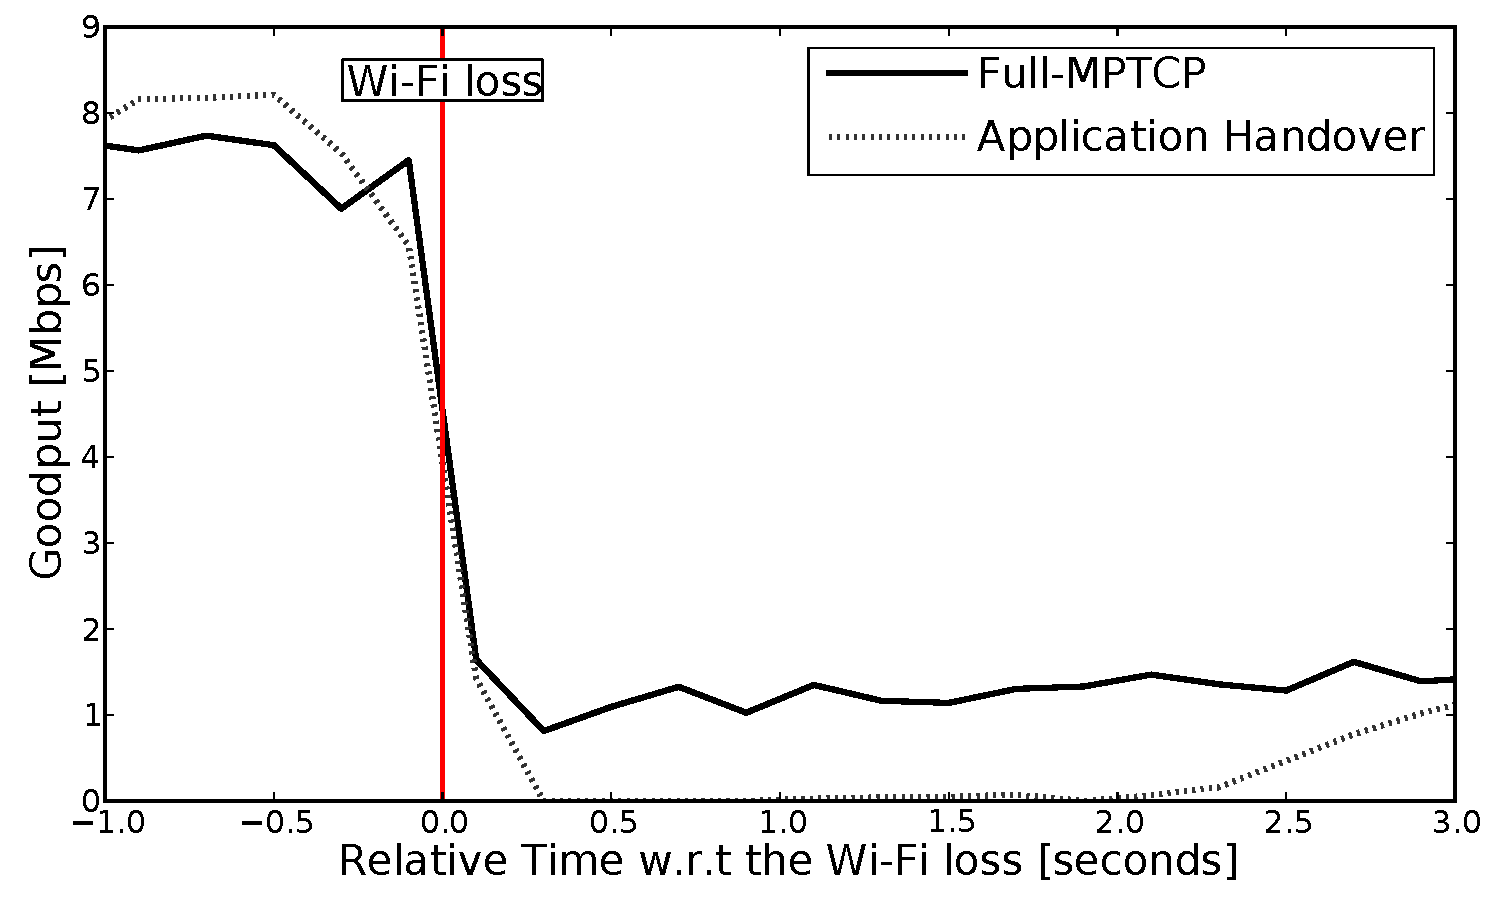
\includegraphics[width=0.7\textwidth]{figures/figure2}
\caption{(Mobility) A mobile device is using both its WiFi and 3G interfaces, and then the WiFi
interface fails. We plot the instantaneous throughputs of Multipath TCP and application-layer
handover. (Reprinted from \cite{Paasch_Mobile:2012}; \copyright 2012,
ACM. Included here by permission.)} 
\label{fig:mptcp2}
\end{figure}

The mobile measurements focus on a typical mode of operation where the device is 
connected to WiFi, the connection goes down and the phone switches to using 3G. 
The setup uses a Linux laptop connected to a WiFi and a 3G network, downloading a 
file using HTTP. 

3G to Wifi handover is implemented in today's phones by changing the application to monitor
the network interfaces. When the app detects the loss of the interface, it creates a new TCP connection 
to the server and the connection can resume. This solution, while simple, is not applicable to all applications
because some of the bytes succesfully delivered by the old connection may be resent by the new one.

Applications that rely on HTTP GET requests (with no side effects) are, however, easy to change. The 
HTTP range header allows a client to resume the download of a file from a specified offset. This is the de-facto
standard for today's apps.  

Figure \ref{fig:mptcp2} compares application layer-handover (with HTTP-range) against Multipath TCP.
The figure shows a 
smooth handover with Multipath TCP, as data keeps flowing despite the interface 
change. With application-layer handover there is a downtime of 4 seconds where the transfer 
stops-this is because it takes time for the application to detect the interface down 
event, and it takes time for 3G to ramp up. 

Multipath TCP enables unmodified mobile applications to survive interface changes with
little disruption. Selected apps can be modified today to support handover, but their performance
is worse than with MPTCP. A more detailed discussion of the utilization of
Multipath TCP in WiFi/3G environments may be found in \cite{Paasch_Mobile:2012}.

\begin{figure}[t]
\centering
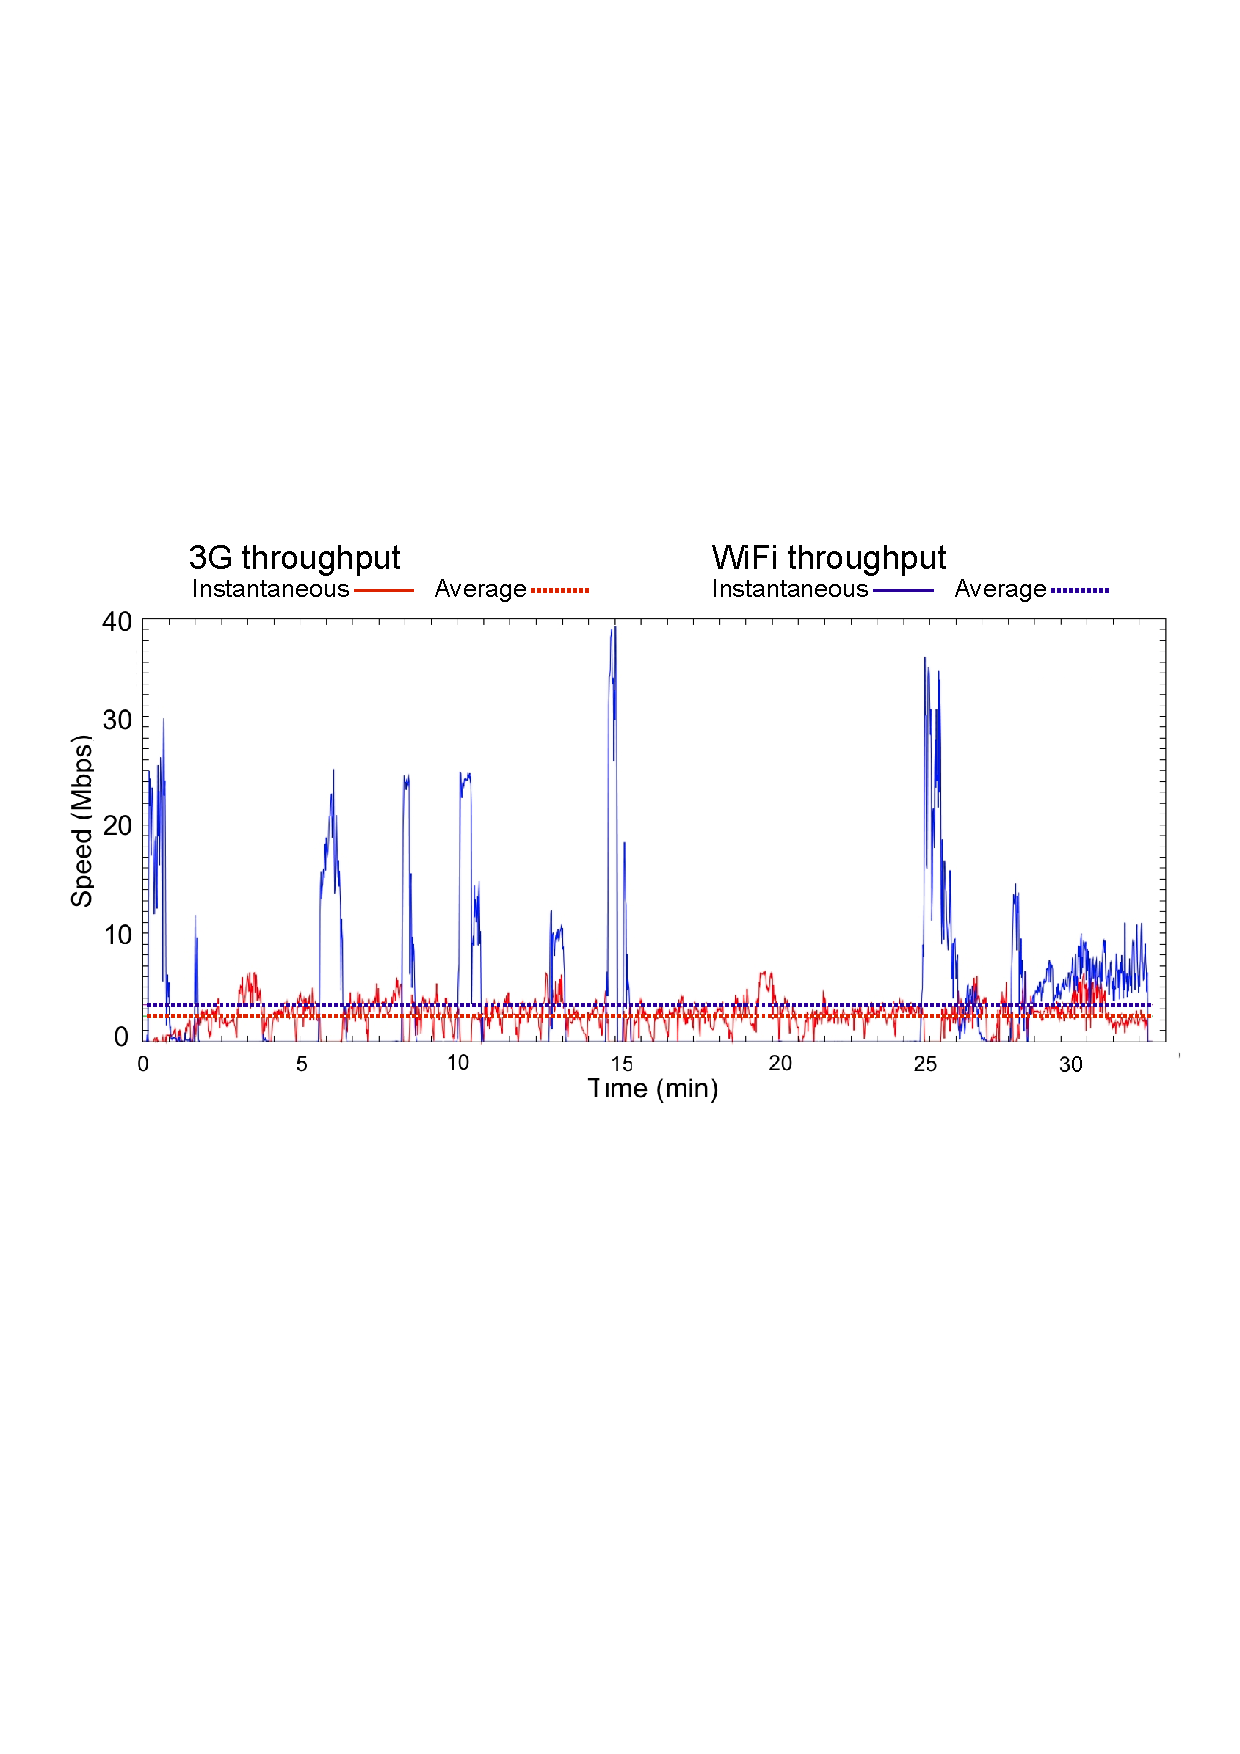
\includegraphics[width=\textwidth,trim=0 11cm 0 9cm,clip=true]{figures/throughput-subway}
\caption{(3G to WiFi Handover) A Linux distribution is downloaded by a mobile user while on the Bucharest subway. 3G coverage is ubiquitous. WiFi is available only in stations.}
\label{fig:throughput-subway}
\end{figure}

We also present a real mobility trace in Figure \ref{fig:throughput-subway}, where a mobile user downloads a Linux distro on his laptop
while travelling on the Bucharest underground. The laptop uses a 3G dongle to connect to the cellular network and its WiFi NIC to connect 
to access points available in stations. 

The figure shows the download speeds of the two interfaces during a 30 minute underground ride. 3G throughput is stable: the average is 
2.3Mbps (shown with a dotted line on the graph), and the instantaneous throughput varies inversely proportional with the distance 
to the 3G cell. WiFi throughput is much more bursty: in some stations the throughput soars to 40Mbps, while in others it is zero, as 
the laptop doesn't manage to associate and obtain an IP address quickly enough. The average WiFi throughput (3.3Mbps) is higher 
than the average 3G throughput.

While MPTCP uses both interfaces in this experiment, using just WiFi when it is available may be preferable as it reduces 3G data bills
and reduces the load of the cellular network. This is easy to implement with MPTCP, as it supports a simple  prioritization mechanism 
that allows the client to inform the server to send data via preferred subflow(s) \footnote{MPTCP sends an MP\_PRIO option to 
inform the remote end about changes in priority for the subflows.}. 


\begin{figure}[t]
\centering
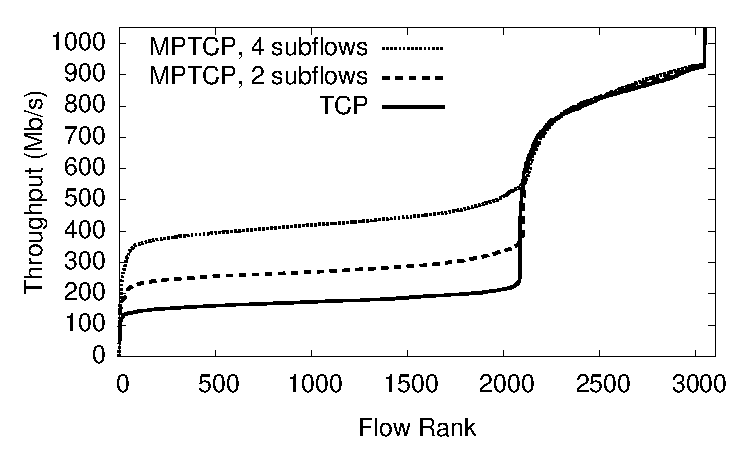
\includegraphics[width=0.5\textwidth]{figures/figure3}
\caption{(Datacenter load-balancing) This graph compares standard TCP with MPTCP 
with two and four flows, when tested on an EC2 testbed with 40 instances. Each host 
uses iperf sequentially to all other hosts. We plot the performance of all flows (Y axis)
in increasing order of their throughputs (X axis). (Reprinted from
\cite{raiciu2011improving}, \copyright ACM, 2011. Included here by permission)}
\label{fig:mptcp3}
\end{figure}

\paragraph{Datacenters.} We also show results from running Multipath TCP in a different scenario: the EC2 datacenter.
Like most datacenters today, EC2 uses a redundant network topology where many paths are 
available between any pair of endpoints, and where connections are placed randomly 
onto available paths. In EC2, 40 machines (or instances) ran the 
Multipath TCP kernel. A simple experiment was run where every machine measured
the throughput sequentially to every other machine using first TCP, then Multipath 
TCP with two and with four subflows. Figure \ref{fig:mptcp3} shows the sorted throughputs measured over 
12 hours. The results show that Multipath TCP brings significant improvements compared 
to TCP in this scenario. Because the EC2 network is essentially a black-box , it is 
difficult to pinpoint the root cause for the improvements; however, a
detailed analysis of the cases where Multipath TCP can help and why in is presented in 
\cite{raiciu2011improving}.

\subsection{Impact of Multipath TCP}

MPTCP is deployable today, as it was designed and shown to work over existing networks and unmodified applications.
Whether MPTCP will be adopted or not is unclear at this point; only time will tell.
If MPTCP is adopted, however, it will likely affect the development of both the network and the applications running 
on top of it. Here we briefly speculate on what the impact might be. 
Multipath TCP embeds two key mechanisms: load balancing to avoid congested paths, and the ability 
to use different IP addresses in the same connection. Having these mechanisms implemented at the end-hosts
means other layers (e.g. the network) may become simpler, and more efficient.

For instance, MPTCP seamlessly uses available bandwidth even if it is short-lived (e.g. WiFi in underground stations), 
and provides robustness when a subset of paths fail by quickly resending data on working paths. This could take
some of the load imposed on BGP, that today must quickly reconverge in the case of a failure. With MPTCP at the endpoints
failures would be ``masked'' automatically, allowing BGP to react to failures slowly which will ensure there are no 
oscillations. However, one must ensure that the paths used by the end-systems are disjoint and that the failure
does not affect all of them.

Another example is layer 2 mobility, implemented in both WiFi and cellular networks, that aims to do a fast handover from 
one access point to the next, or from one cell to the next. With MPTCP as a transport protocol, a WiFi client could connect
simultaneously to two access points or cells (provided the L2 protocol allows it), and load balance traffic on the best 
link. MPTCP could replace fast handovers with slow handovers that are more robust. Of course, some changes may be needed 
at layer 2 to support such load balancing.

Network topologies may be designed differently if MPTCP is the transport protocol. An example is GRIN \cite{grin}, a work that
proposes to change existing datacenter networks by randomly interconnecting servers in the same rack directly, using their free 
NIC ports. This allows a server to opportunistically send traffic at speeds larger than its access link by having its idle neighbor 
relay some traffic on its behalf. With a minor topology change and MPTCP, GRIN manages to better utilize the datacenter network core.

The mechanisms that allow MPTCP to use different IPs in the same transport connection (i.e. the connection identifier) 
also allow connections to be migrated across physical machines with different IP addresses. One direct application is seamless virtual
machine migration: an MPTCP-enabled guest virtual machine can just resume its connections after it is migrated.

On the application side many optimizations are possible. Applications like video
and audio streaming only need a certain bitrate to ensure user satisfaction - they rarely fully utilize the wireless capacity.
Our mobility graph in the previous section shows that, in principle, WiFi has enough capacity to support these apps, even if it is 
only available in stations. A simple optimization would be to download as much of the video as possible while on WiFi, and only
use 3G when the playout buffer falls below a certain threshold. This would ensure a smooth viewing experience while pushing as 
much traffic as possible over WiFi. 

The examples shown in this section are only meant to be illustrative, and their potential impact or even feasibility 
is not clear at this point. Further, the list is not meant to be exhaustive. 
We have only provided it to show that Multipath TCP benefits go beyond than
increasing throughput, and could shape both the lower and the upper layers of the protocol stack in the future.
